\documentclass[tikz,border=10pt]{standalone}
\usetikzlibrary{calc}
\begin{document}
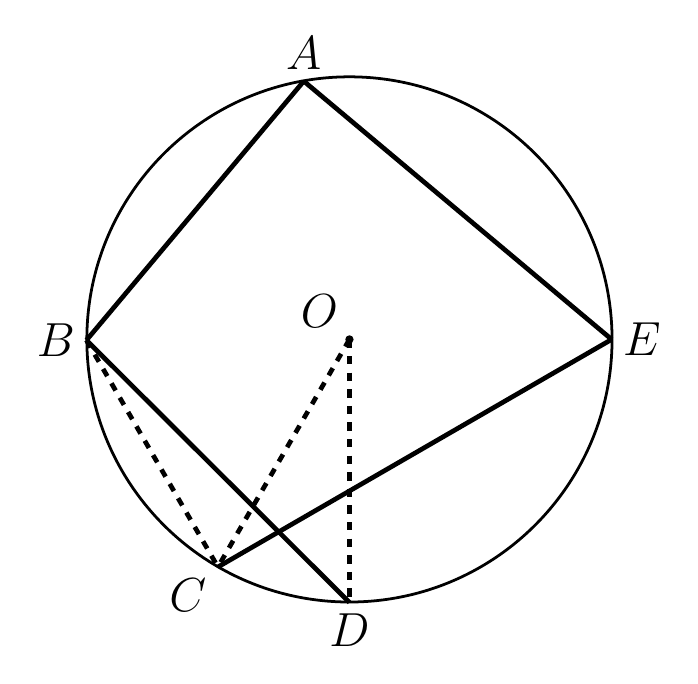
\begin{tikzpicture}[line join=round, line width=1.7pt]

% Named coordinates (TikZ units in cm, s = 0.02122, origin at O)
\coordinate (O) at (0,0);
\coordinate (A) at (-0.58,3.28);
\coordinate (B) at (-3.34,-0.01);
\coordinate (E) at (3.33,0);
\coordinate (C) at (-1.67,-2.89);
\coordinate (D) at (0,-3.34);
\coordinate (P) at (-0.90,-2.45);   % BD ∩ EC (reference only)
\coordinate (Q) at (-1.22,-2.13);   % BD ∩ OC (reference only)
\coordinate (R) at (0,-1.93);       % EC ∩ OD (reference only)

% Circle: bolder black stroke (1pt)
\draw[black, line width=1pt] (O) circle (3.335);

% Solid chords
\draw (A) -- (B);
\draw (A) -- (E);
\draw (B) -- (D);
\draw (E) -- (C);

% Dashed auxiliaries (OC runs exactly C to O)
\draw[dashed] (O) -- (C);
\draw[dashed] (B) -- (C);
\draw[dashed] (O) -- (D);

% Centre point: filled dot and label
\fill (O) circle (1.5pt);
\node[above left] at (O) {\fontsize{17}{20.4}\selectfont $O$};

% Vertex labels
\node[above] at (A) {\fontsize{17}{20.4}\selectfont $A$};
\node[left] at (B) {\fontsize{17}{20.4}\selectfont $B$};
\node[right] at (E) {\fontsize{17}{20.4}\selectfont $E$};
\node[below left] at (C) {\fontsize{17}{20.4}\selectfont $C$};
\node[below] at (D) {\fontsize{17}{20.4}\selectfont $D$};

\end{tikzpicture}
\end{document}